\subsection{Descripci\'on del problema}

Nos encontramos ante una competencia que consiste en cruzar un puente dando saltos con la menor cantidad posible de estos.
Cada participante tiene una capacidad de salto o salto máximo limitado, razón por la cual no pueden cruzar el puente de un salto, a menos que su salto sea mayor a la longitud del puente. Esta longitud la medimos por la cantidad de tablones que posee el puente.
Para no hacer demasiado trivial la competencia, no todos los tablones del puente están en buen estado, algunos están rotos, pero están marcados para que no se salte a estos. Esto trae una consecuencia, puede darse el caso que el salto máximo de un participante sea n y en el puente haya m tablones rotos continuos, con m > n, por lo tanto cuando el participante llegue al tablón anterior a esta serie continua de tablones rotos, no podrá efectuar mas saltos, y pierde el juego. 

\subsection{Resoluci\'on}


\subsection{Demostraci\'on de la resoluci\'on}


\subsection{Complejidad del algoritmo}


\subsection{C\'odigo fuente}

\lstset{language=C++,
                basicstyle=\ttfamily\footnotesize,
                keywordstyle=\color{blue}\ttfamily,
                stringstyle=\color{red}\ttfamily,
                commentstyle=\color{green}\ttfamily,
                morecomment=[l][\color{magenta}]{\#},
                breaklines=true
}
\begin{lstlisting}

typedef std::vector<int> LTablonesEstado;
typedef std::vector<int> LSaltos;

LSaltos resolver(int cantTablones, int saltoMaximo, LTablonesEstado& tablones){

	LSaltos saltos;
	int contadorSaltoMaximo = 0;
	int tablonASaltar;
	int tamSalto = 0;
	bool encontroSalto = false;

	for(int nroTablon = 0; nroTablon < cantTablones; nroTablon++){

		contadorSaltoMaximo++;
		tamSalto++;
		
		//Si hay un tablon en ese lugar actualizo tablonASaltar
		if(tablones[nroTablon] == 1){
			tablonASaltar = nroTablon;
			encontroSalto = true;
		}
		
		//Si llegue al limite de salto agrego (Y pude hacer un salto) agrego el tablon al que voy a saltar a la lista de saltos y reinicio los contadores
		if(contadorSaltoMaximo == saltoMaximo && encontroSalto){			
			//Guardo el tablon al que salte
			saltos.push_back(tablonASaltar);

			//reinicio las variables para un nuevo salto
			contadorSaltoMaximo = saltoMaximo - tamSalto;
			tamSalto = 0;
			encontroSalto = false;

		}else if (contadorSaltoMaximo == saltoMaximo && !encontroSalto)
		{
			saltos.clear();
			break;
		}
	}
	return saltos;//Tambien devolver si se pudo llegar al final con saltos.
}

\end{lstlisting}

\subsection{Casos de prueba}

Para este ejercicio escogimos algunos casos de prueba que tienen las siguientes características:

\begin{itemize}

\item Caso en el que el puente no posee ningún tablón roto. Aquí el participante debería cruzar el puente dando saltos de tamaño igual a su salto máximo, ya que no hay nada que impida que no lo haga.

\item Caso en el que el puente no posee tablones sanos, y el limite de salto del jugador es menor a la cantidad de tablones del puente. El participante no podrá hacer ningún salto, ya que no importa de que longitud sea este, siempre terminará cayendo en un tablón roto.

\item Caso en el que el puente no posee tablones sanos, y el limite de salto del jugador es mayor a la cantidad de tablones del puente. En este caso el participante podrá cruzar el puente de un salto igual al tamaño del puente mas uno.

\item Caso en el que los tablones sanos están cada $x$ tablones, donde $x$ es igual al salto máximo del participante. En este caso el participante cruzara el puente en $m$ cantidad de saltos, donde $m$ es la cantidad de tablones sanos. Osea que pasará por todos los tablones sanos.

\item Caso en el cual los últimos $m$ tablones están rotos, por lo tanto el algoritmo debe ejecutarse con normalidad, pero a la hora de evaluar el ultimo salto, este no podrá efectuarse y se debe borrar la lista de saltos hechos y retornar "no".

\end{itemize}


\subsection{Performance}

Para realizar el testeo de performance creamos test.cpp, el cual genera casos de test pseudo-aleatorios determinados por una semilla, la cual se pasa como parámetro al ejecutable 'test', por ejemplo: ./test 6

Este crea 150 casos de prueba con una cantidad de tablones del puente entre 1 y 100000000, llamemoslo $n$, y un salto máximo, $s$, entre 1 y $n$ y el valor de cada tablón, todos, como ya dijimos, pseudo-aleatorios.

Para comenzar, modificamos el archivo test.cpp para genere 20 pruebas con 20 tamaños de puente diferentes, escogidos de la manera descrita, y realice sobre cada uno de estos 100 ejecuciones del algoritmo variando el valor $s$ (salto máximo).
Esto lo hicimos para corroborar y tratar de probar empíricamente que, como esta explicado en el punto de Resolución, la complejidad del algoritmo depende puramente de la cantidad de tablones del puente, $n$, y no posee ninguna dependencia con el valor de $s$.
Los resultados los guardamos en el archivo testSaltoMaximo.out, los cuales graficamos obteniendo lo siguiente:


\begin{figure}[h]
\begin{center}
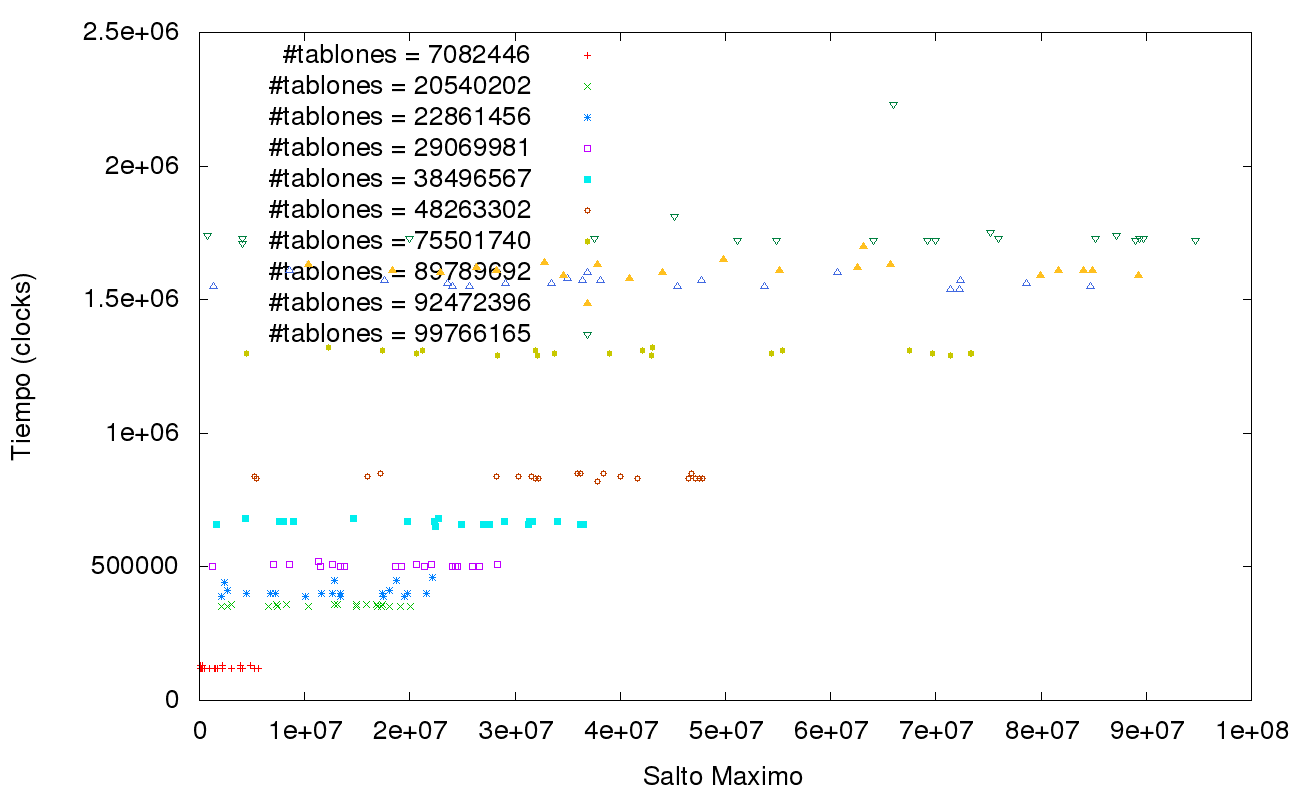
\includegraphics[scale=1]{./imagenes/ej1_testSaltoMaximo.png}
\caption{Gr\'afico de tiempo en funci\'on del salto m\'aximo.}
\end{center}
\end{figure}


Como puede observarse el tiempo de ejecución de cada uno de los 20 test variando $n$, es constante en la variación de $s$, con un desvío estándar muy pequeño, el cual puede darse por un dos de factores: 
*Al cambiar el tamaño de salto es muy posible que en algunos casos el algoritmo termine satisfactoriamente, encontrando una solución, pero en otros casos puede que el salto máximo sea mas chico que la mayor cantidad de tablones rotos continuos $c$, osea que $s$ < $c$. En este caso el algoritmo termina al no poder saltar.
*Al medir el tiempo de clock nuestro proceso no corre solo en la arquitectura que lo testeamos, hay otros procesos ejecutándose, por lo que la misma corrida puede dar algún tiempo de diferencia.
Y con esto concluimos que $s$ no afecta la complejidad temporal del algoritmo.

A continuación corrimos 'test' con 3 semillas distintas: 1, 2 y 3, para ahora si, empíricamente mostrar que la complejidad del algoritmo es O(n)
Esto lo hicimos 10 veces, para poder promediar los tiempos de ejecución, por los motivos arriba enumerados, razón por la cual podríamos obtener tiempo de ejecución mayor al real. Y porque al correr 10 veces seguidas un mismo test, el procesador podría llegar a cachear algunos resultados, dándonos un tiempo de ejecución menor al real.
Una vez obtenidos estos promedios, graficamos los resultados de los 3 test junto con una representación lineal de $n$,para esto calculamos $t$ $/$ $n$ (El promedio de la esta división en todos los test dio aproximadamente 0.17) para así obtener la constante por la cual podemos multiplicar $n$ y poder compararlos gráficamente de una forma más simple de analizar.  De esta forma obtuvimos el siguiente gráfico:

\begin{figure}[h]
\begin{center}
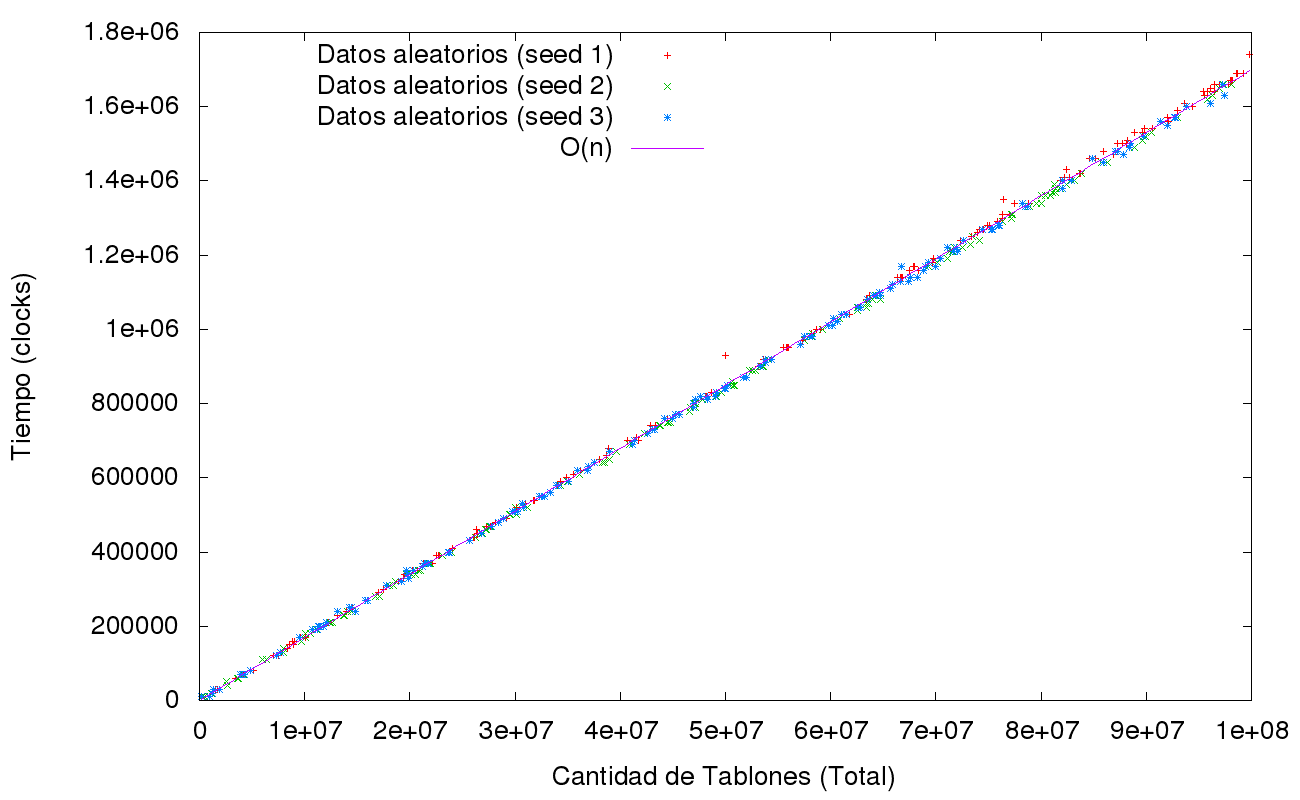
\includegraphics[scale=0.4]{./imagenes/ej1_chartRendimiento.png}
\caption{Gr\'afico de tiempos con test pseudo-aleatorios.}
\end{center}
\end{figure}

Se puede observar que el valor $t$ es lineal es totalmente lineal, tal como queríamos mostrar.
